\documentclass{acm_proc_article-sp}
\begin{document}
\title{Bar Dude \\ An Interactive Bar}
\numberofauthors{4} 
\author{
\alignauthor
Nicolas Erbach\\
       \email{s9nierba@stud.uni-saarland.de}
\alignauthor
Tobias Kiefer\\
       \email{s9tskief@stud.uni-saarland.de}
       \and  
\alignauthor Maike Maas\\
       \email{s9memaas@stud.uni-saarland.de}
\alignauthor Manuel Zapp\\
       \email{s9mazapp@stud.uni-saarland.de}
}
\date{25 September 2015}

\maketitle
\begin{abstract}

\end{abstract}



\section{Introduction}


\section{Concept}
\subsection{Idea}
The idea behind Bar Dude is a cocktail bar that guides people through the single steps of mixing their favourite cocktails. In a first step you are able to choose a cocktail on the website of the bar by connecting to it with your smart phone or laptop. In a second step it supports each client by illuminating the ingredients of the cocktail he or she selected step by step and by giving clear advice when you put enough of the single ingredients into the cocktail.
\subsection{Approach}

\begin{figure}[htbp] 
  \centering
     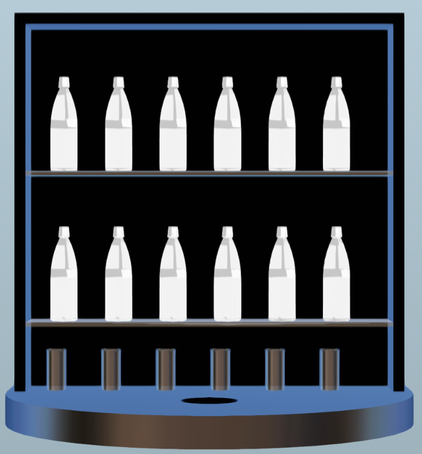
\includegraphics[width=0.5\linewidth]{pictures/bar_inventor.png}
  \caption{Sketch of the bar}
  \label{fig:bar_inventor}
\end{figure}

\begin{figure}[htbp] 
  \centering
     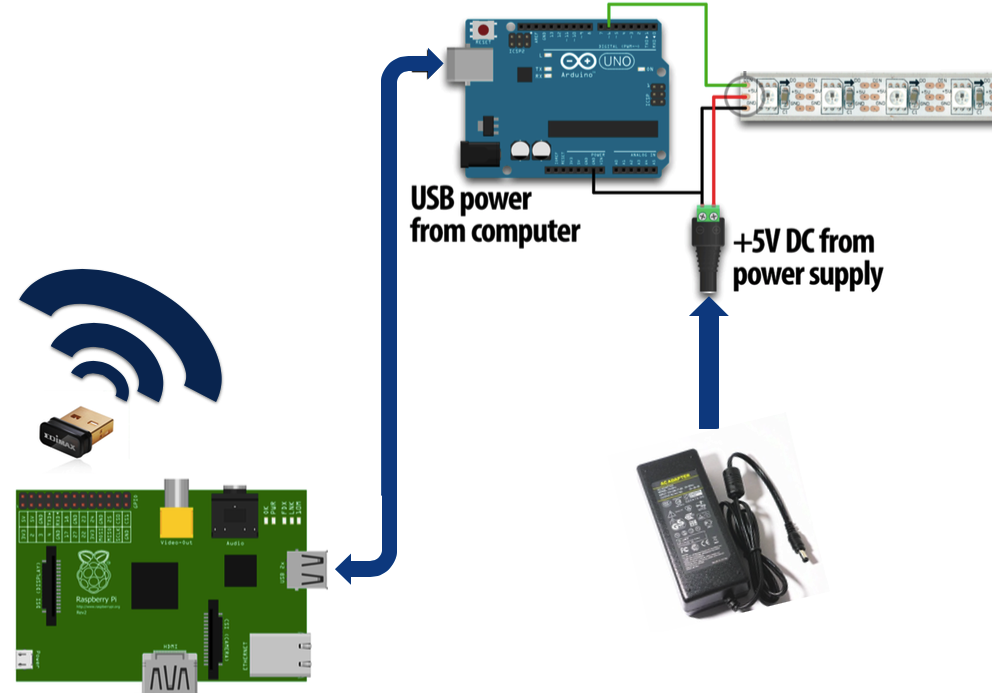
\includegraphics[width=0.7\linewidth]{pictures/technical.png}
  \caption{Technical specification}
  \label{fig:technical}
\end{figure}

\section{Hardware Construction}
\subsection{Woodwork}
After planning the rack and the shelves of the bar, we calculated the amount of wood we would need to build it. In a next step we had to cut the wood we bought into the right pieces. For the rounding of the rack bottom we contacted a local carpenter since we did not have the right instruments for doing this difficult cuts properly. The other small pieces were cut with a buzz saw as you can see in figure \ref{fig:cutting_wood}.

\begin{figure}[htbp] 
  \centering
     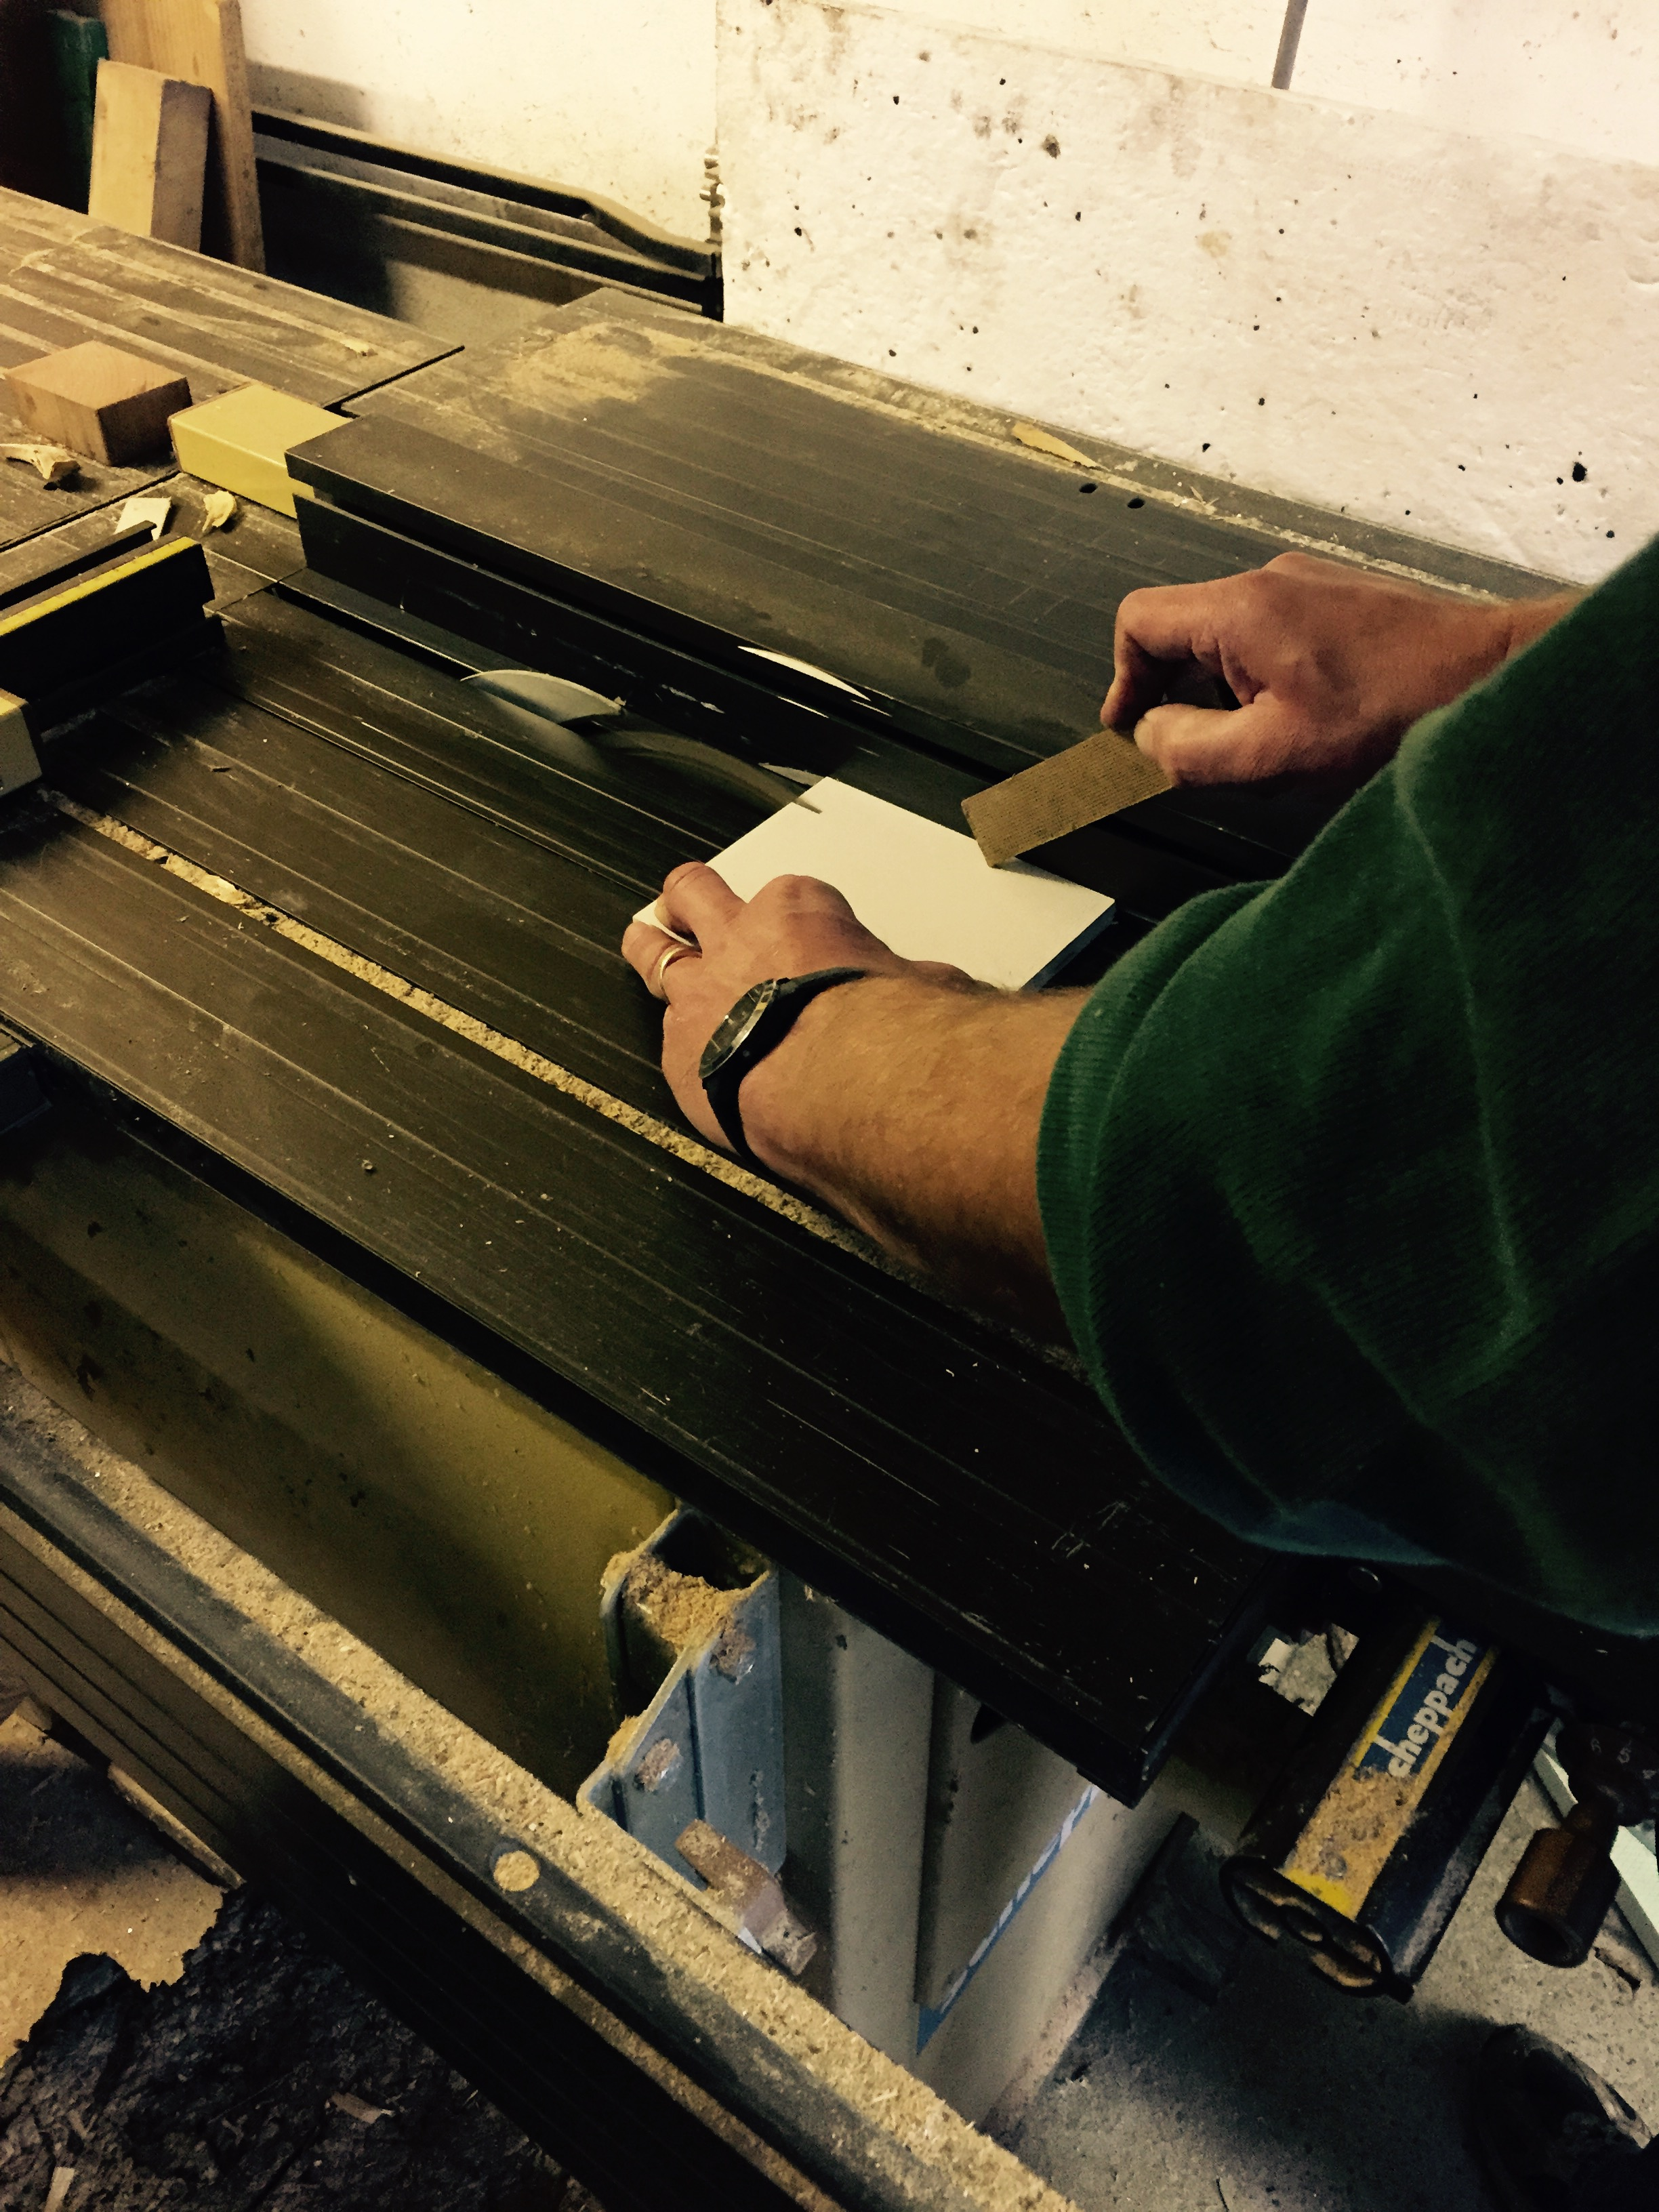
\includegraphics[width=0.5\linewidth]{pictures/cutting_wood.jpg}
  \caption{Cutting of the wood}
  \label{fig:cutting_wood}
\end{figure}

When all pieces of the rack were fitted, we started to assemble the rack. Therefore we used screws and wood glue so that the bar would keep stable. Figure \ref{fig:assembling} shows how the base plate is screwed together.

\begin{figure}[htbp] 
  \centering
     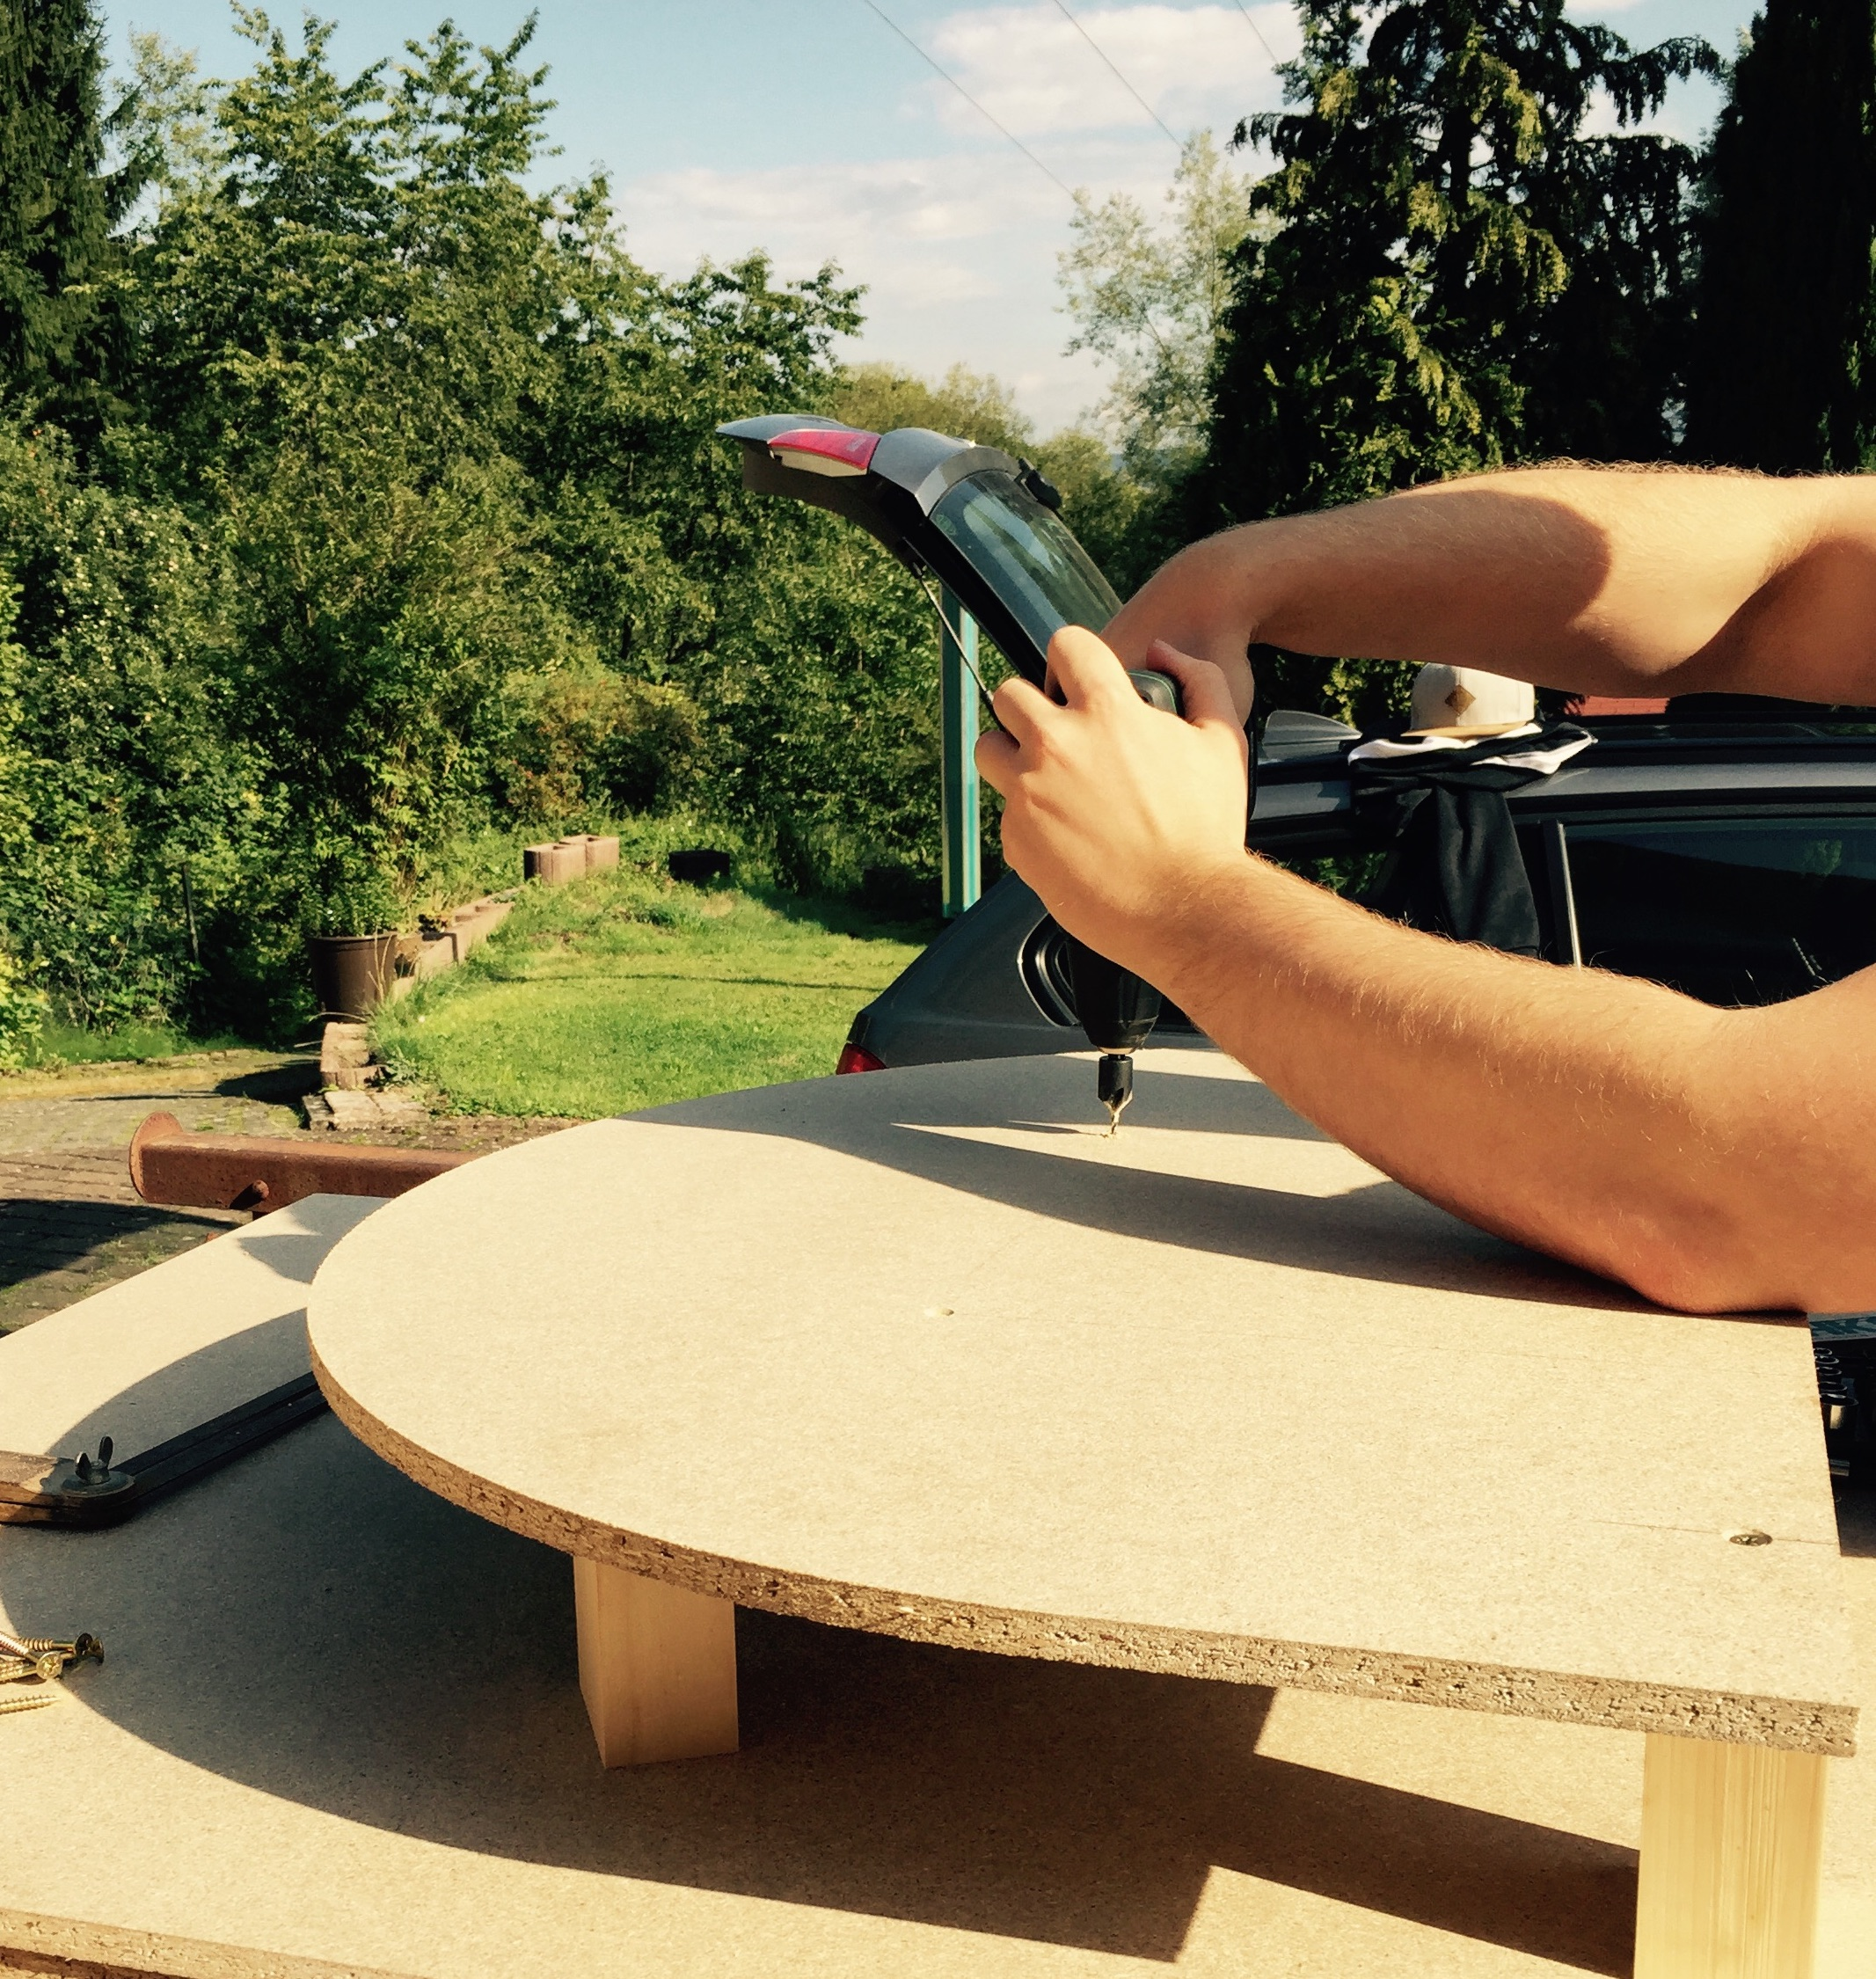
\includegraphics[width=0.5\linewidth]{pictures/assembling.jpg}
  \caption{Assembling of the rack}
  \label{fig:assembling}
\end{figure}

The finished framing of the rack is shown in figure \ref{fig:framing}. This picture also illustrates that we did the panelling between the two base plates with 4 mm poplar wood because this is to thin and flexible that it can be bend.

\begin{figure}[htbp] 
  \centering
     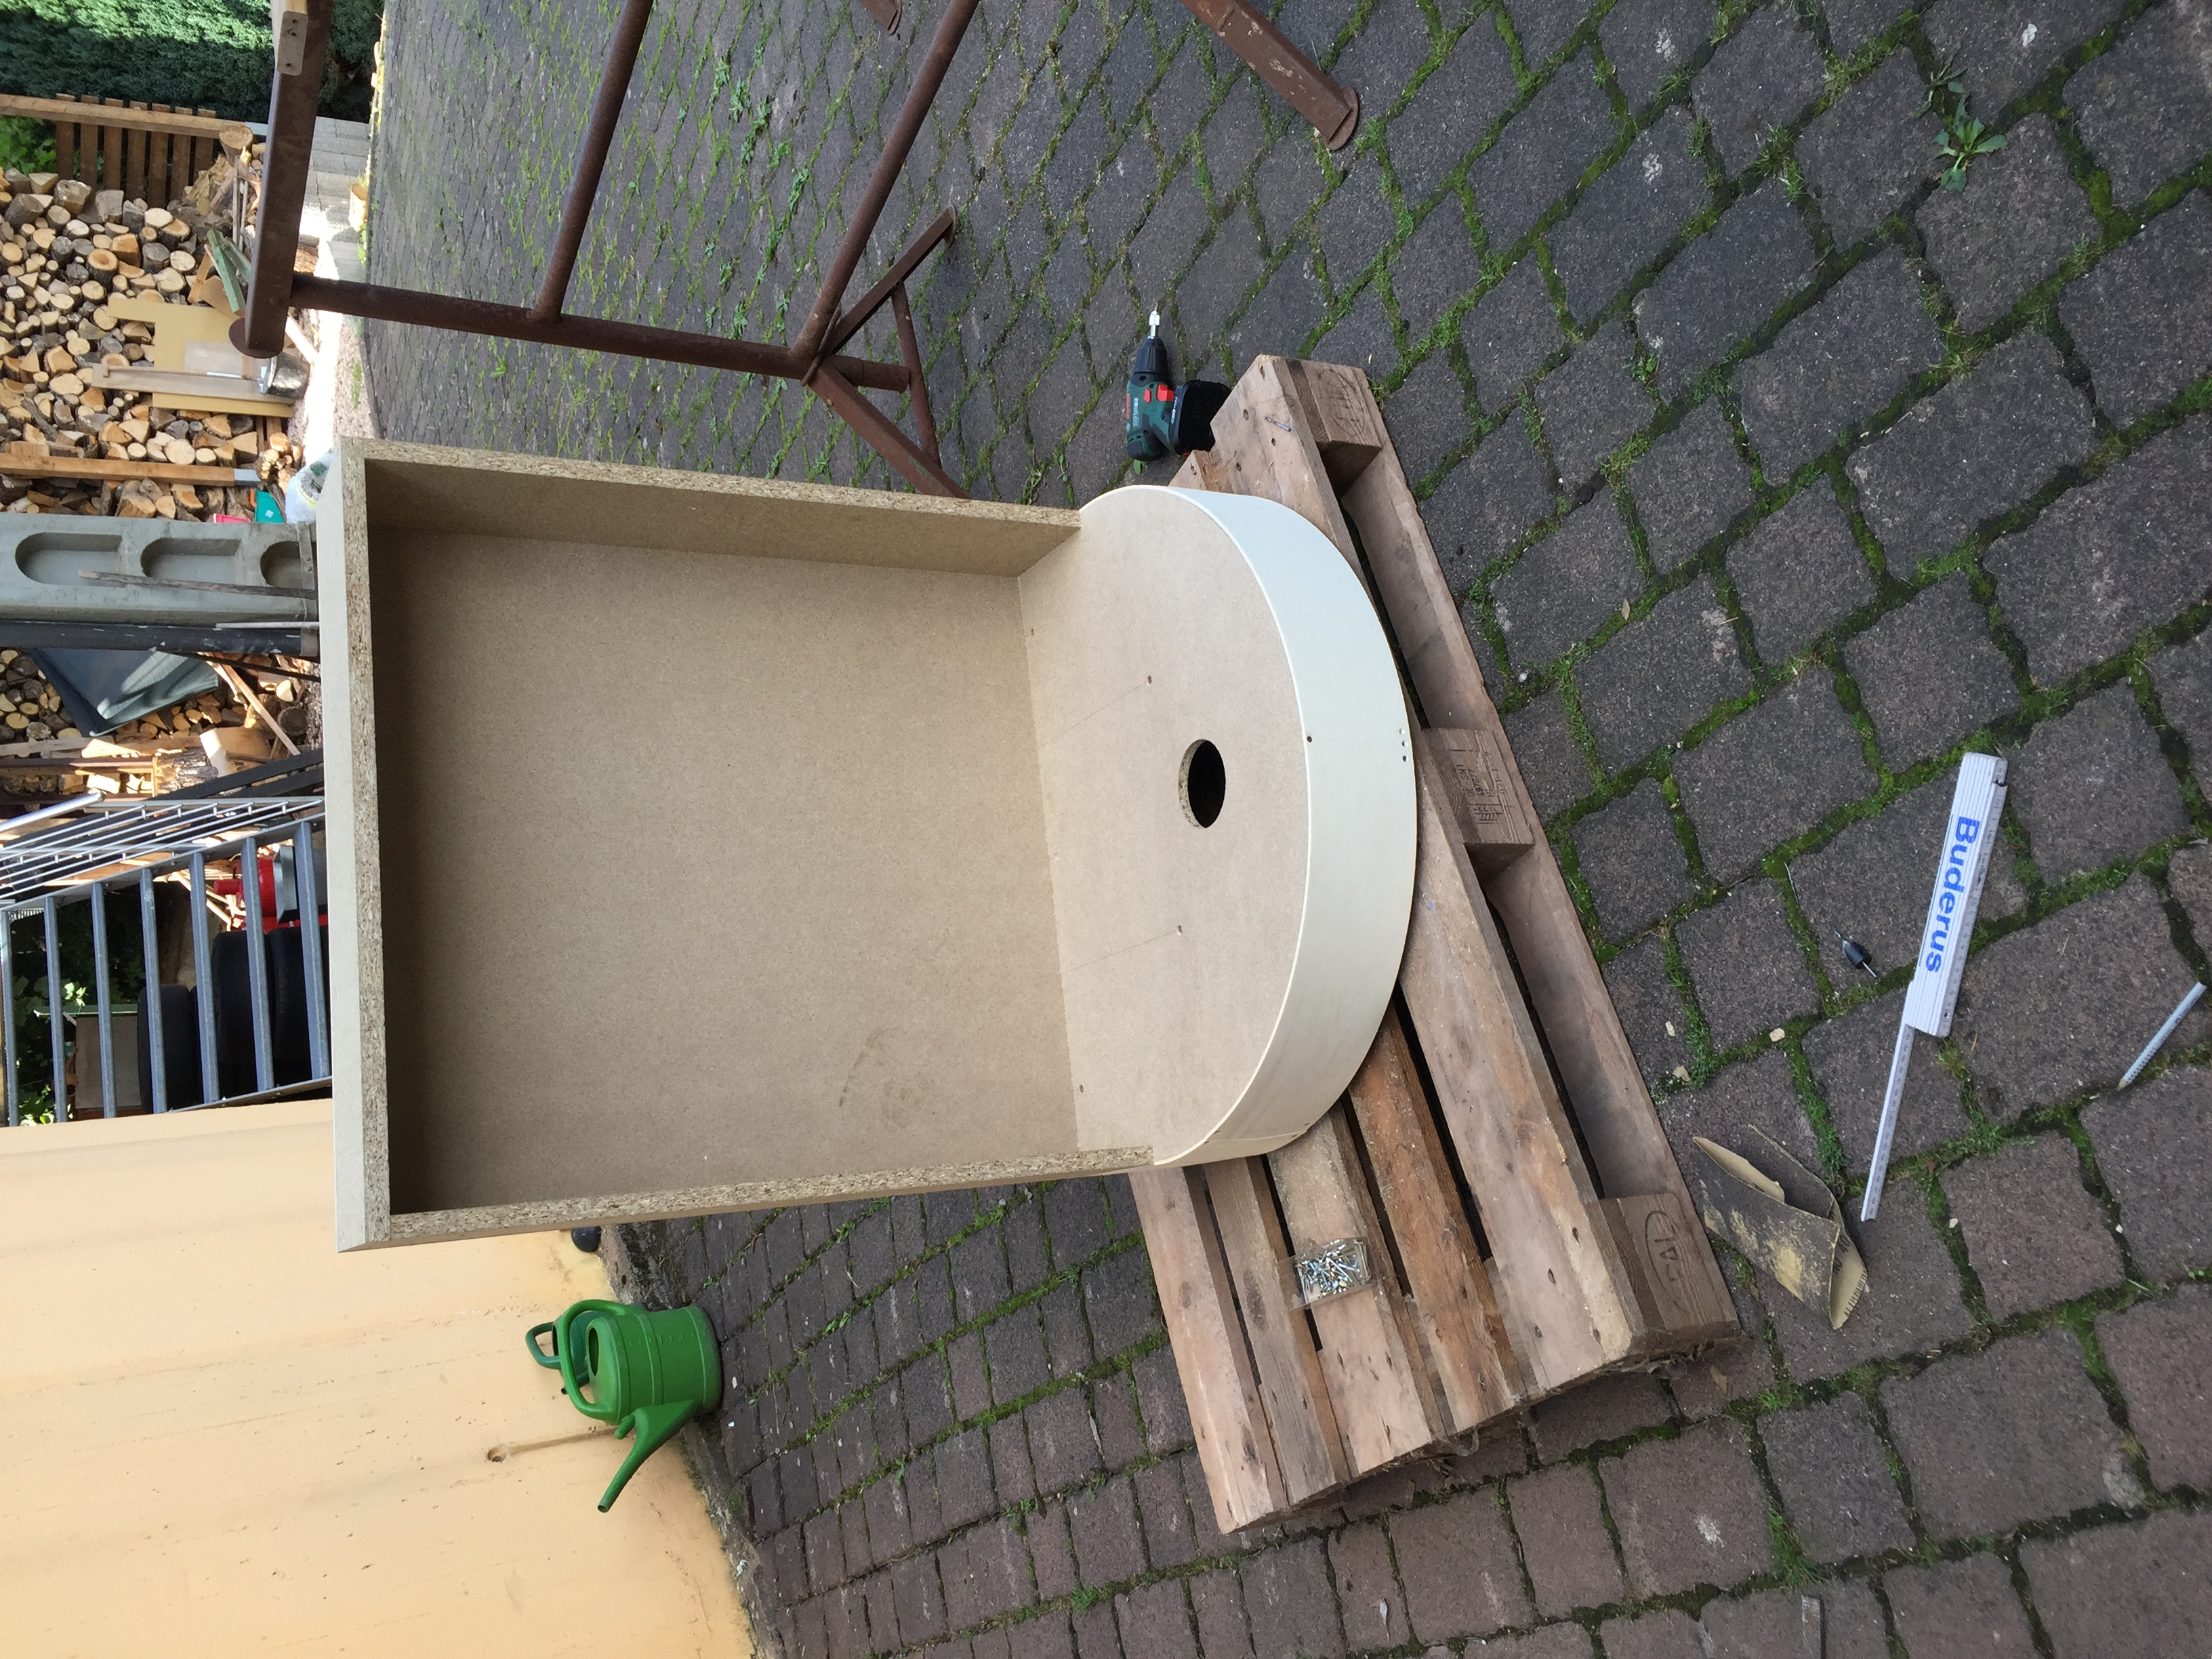
\includegraphics[width=0.6\linewidth, angle =270]{pictures/rack2.jpg}
  \caption{Framing of the rack}
  \label{fig:framing}
\end{figure}

For deriving a smooth surface of the rack, we filled all screw wholes with filler. Since we used plywood, we also filled the edges of the rack, so that it is easier to prime and paint the bar. 

\begin{figure}[htbp]  
  \centering
     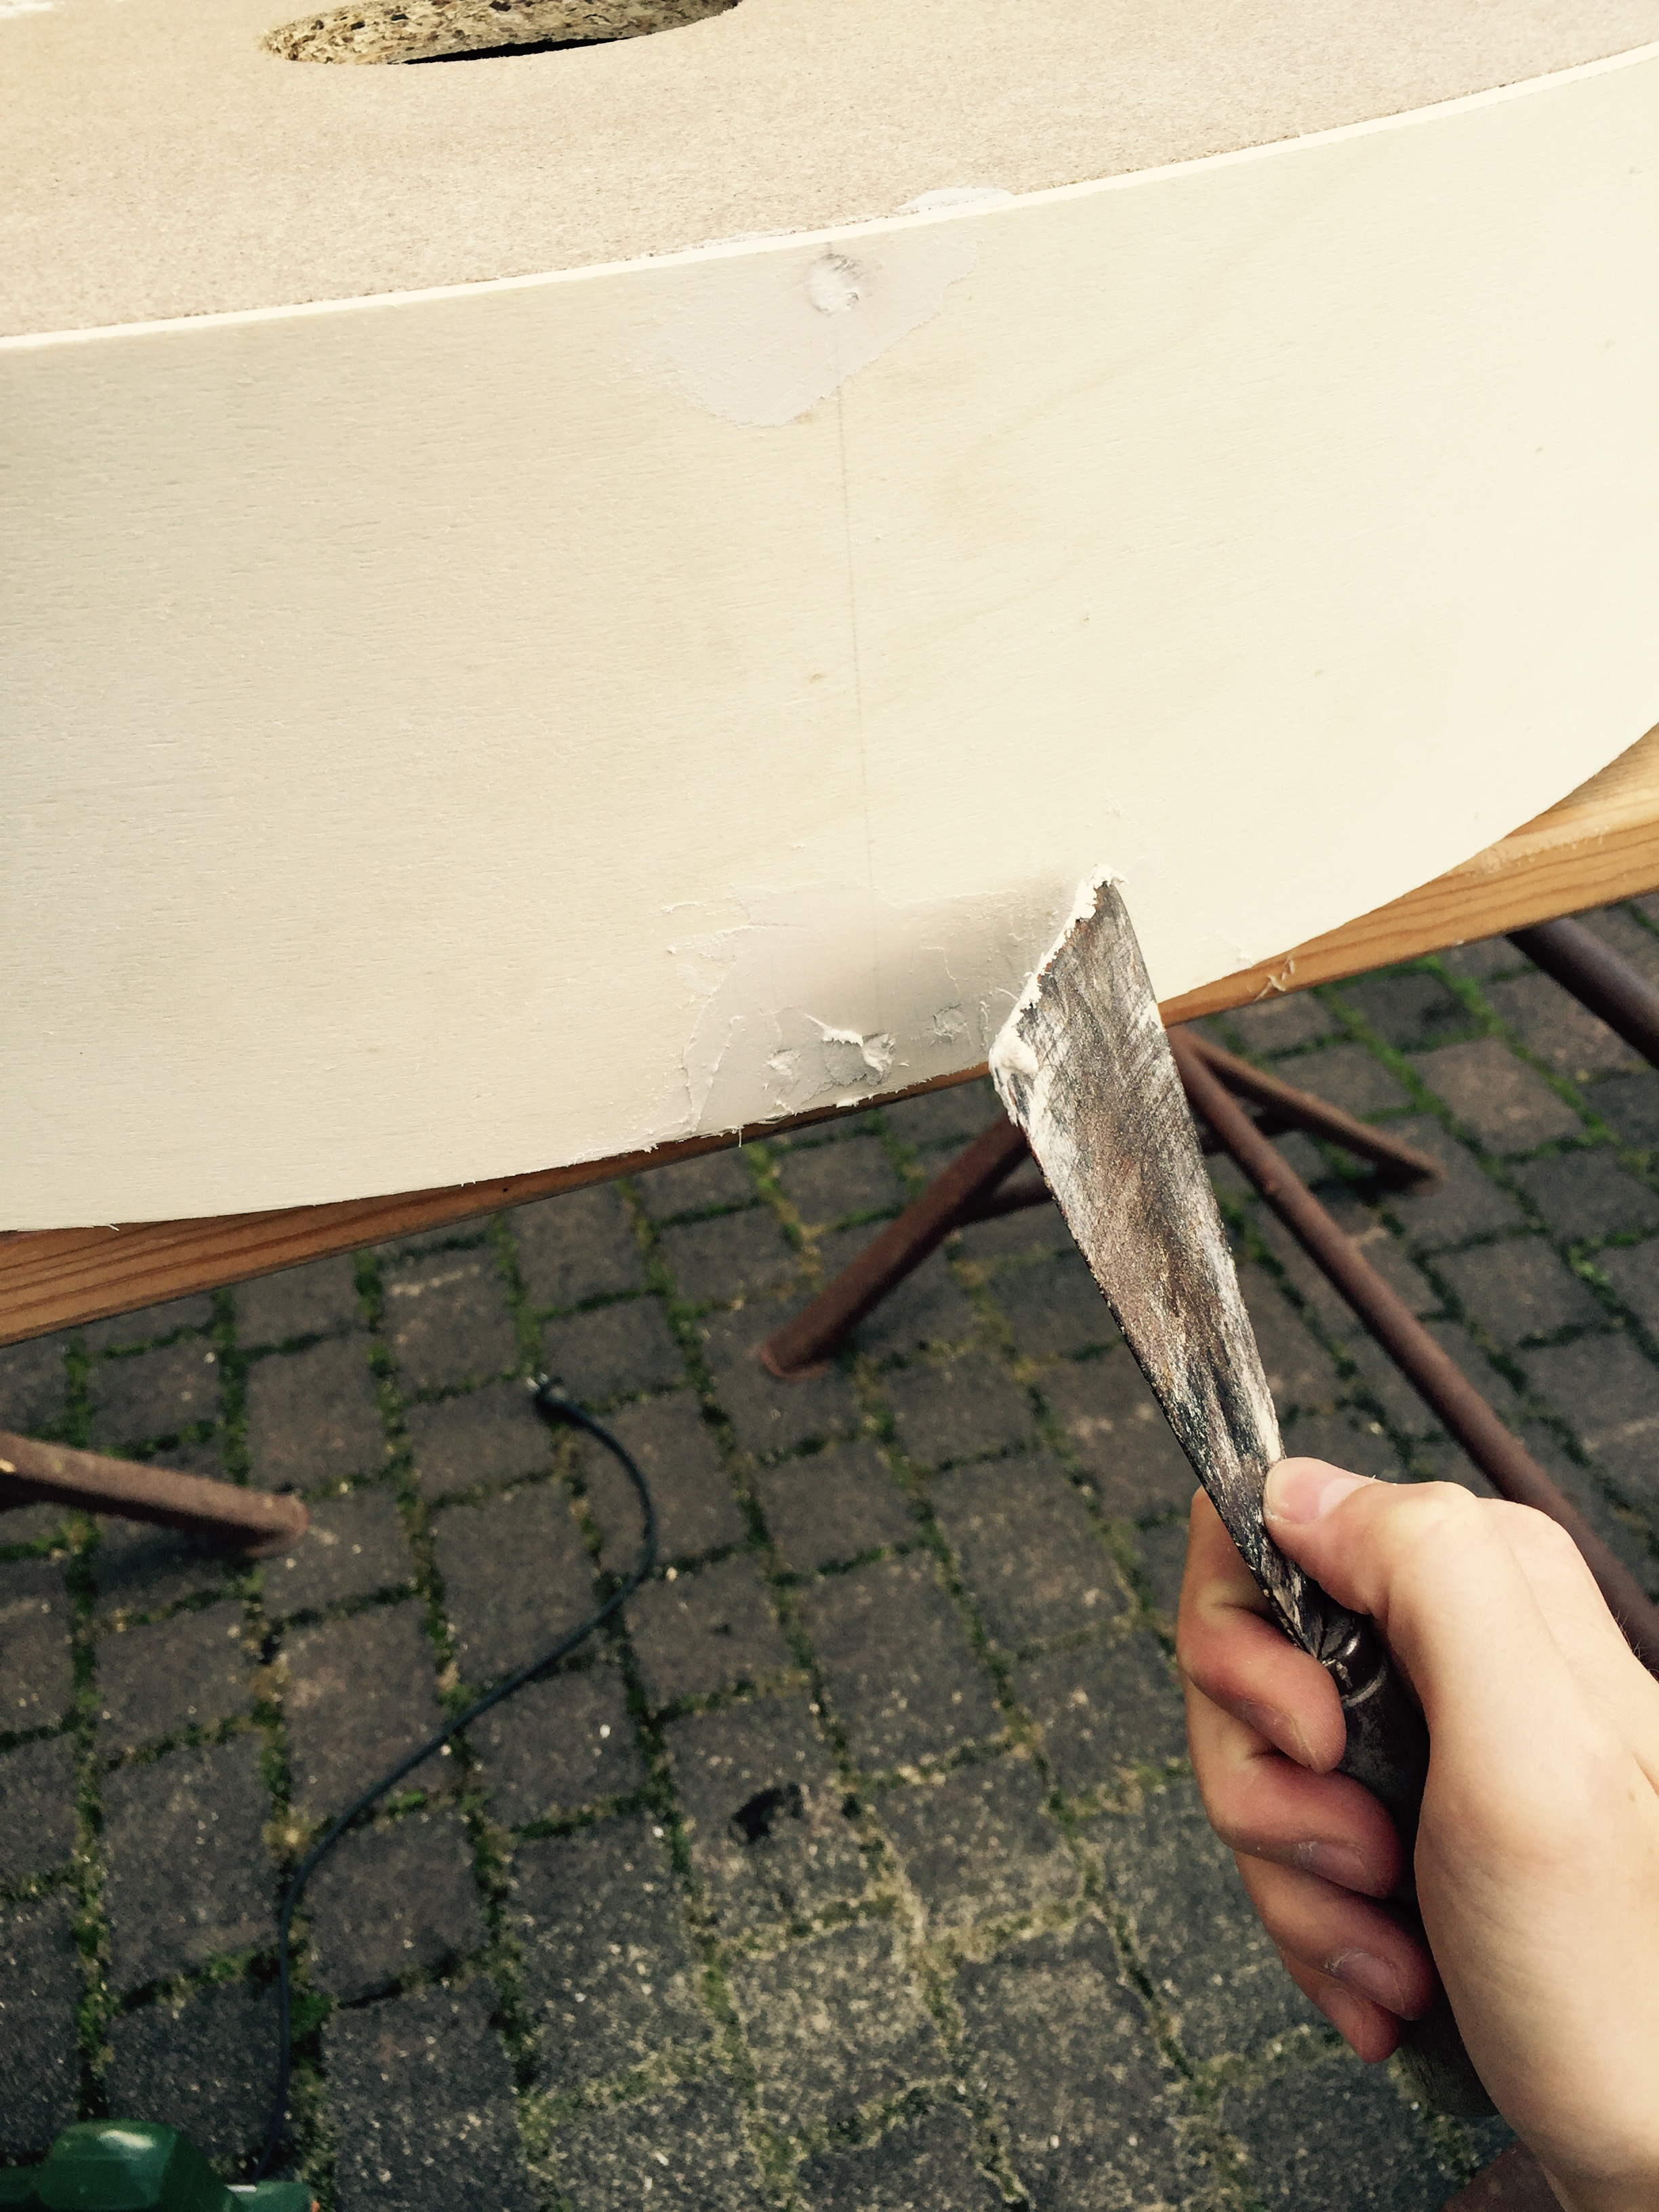
\includegraphics[width=0.5\linewidth]{pictures/filling.jpg}
  \caption{Filling of the screw wholes}
  \label{fig:filling}
\end{figure}

In a next step we polished the bar since had to remove the needless filler and roughen the wood. This work step can be seen in figure \ref{fig:polishing}
 
\begin{figure}[htbp] 
  \centering
     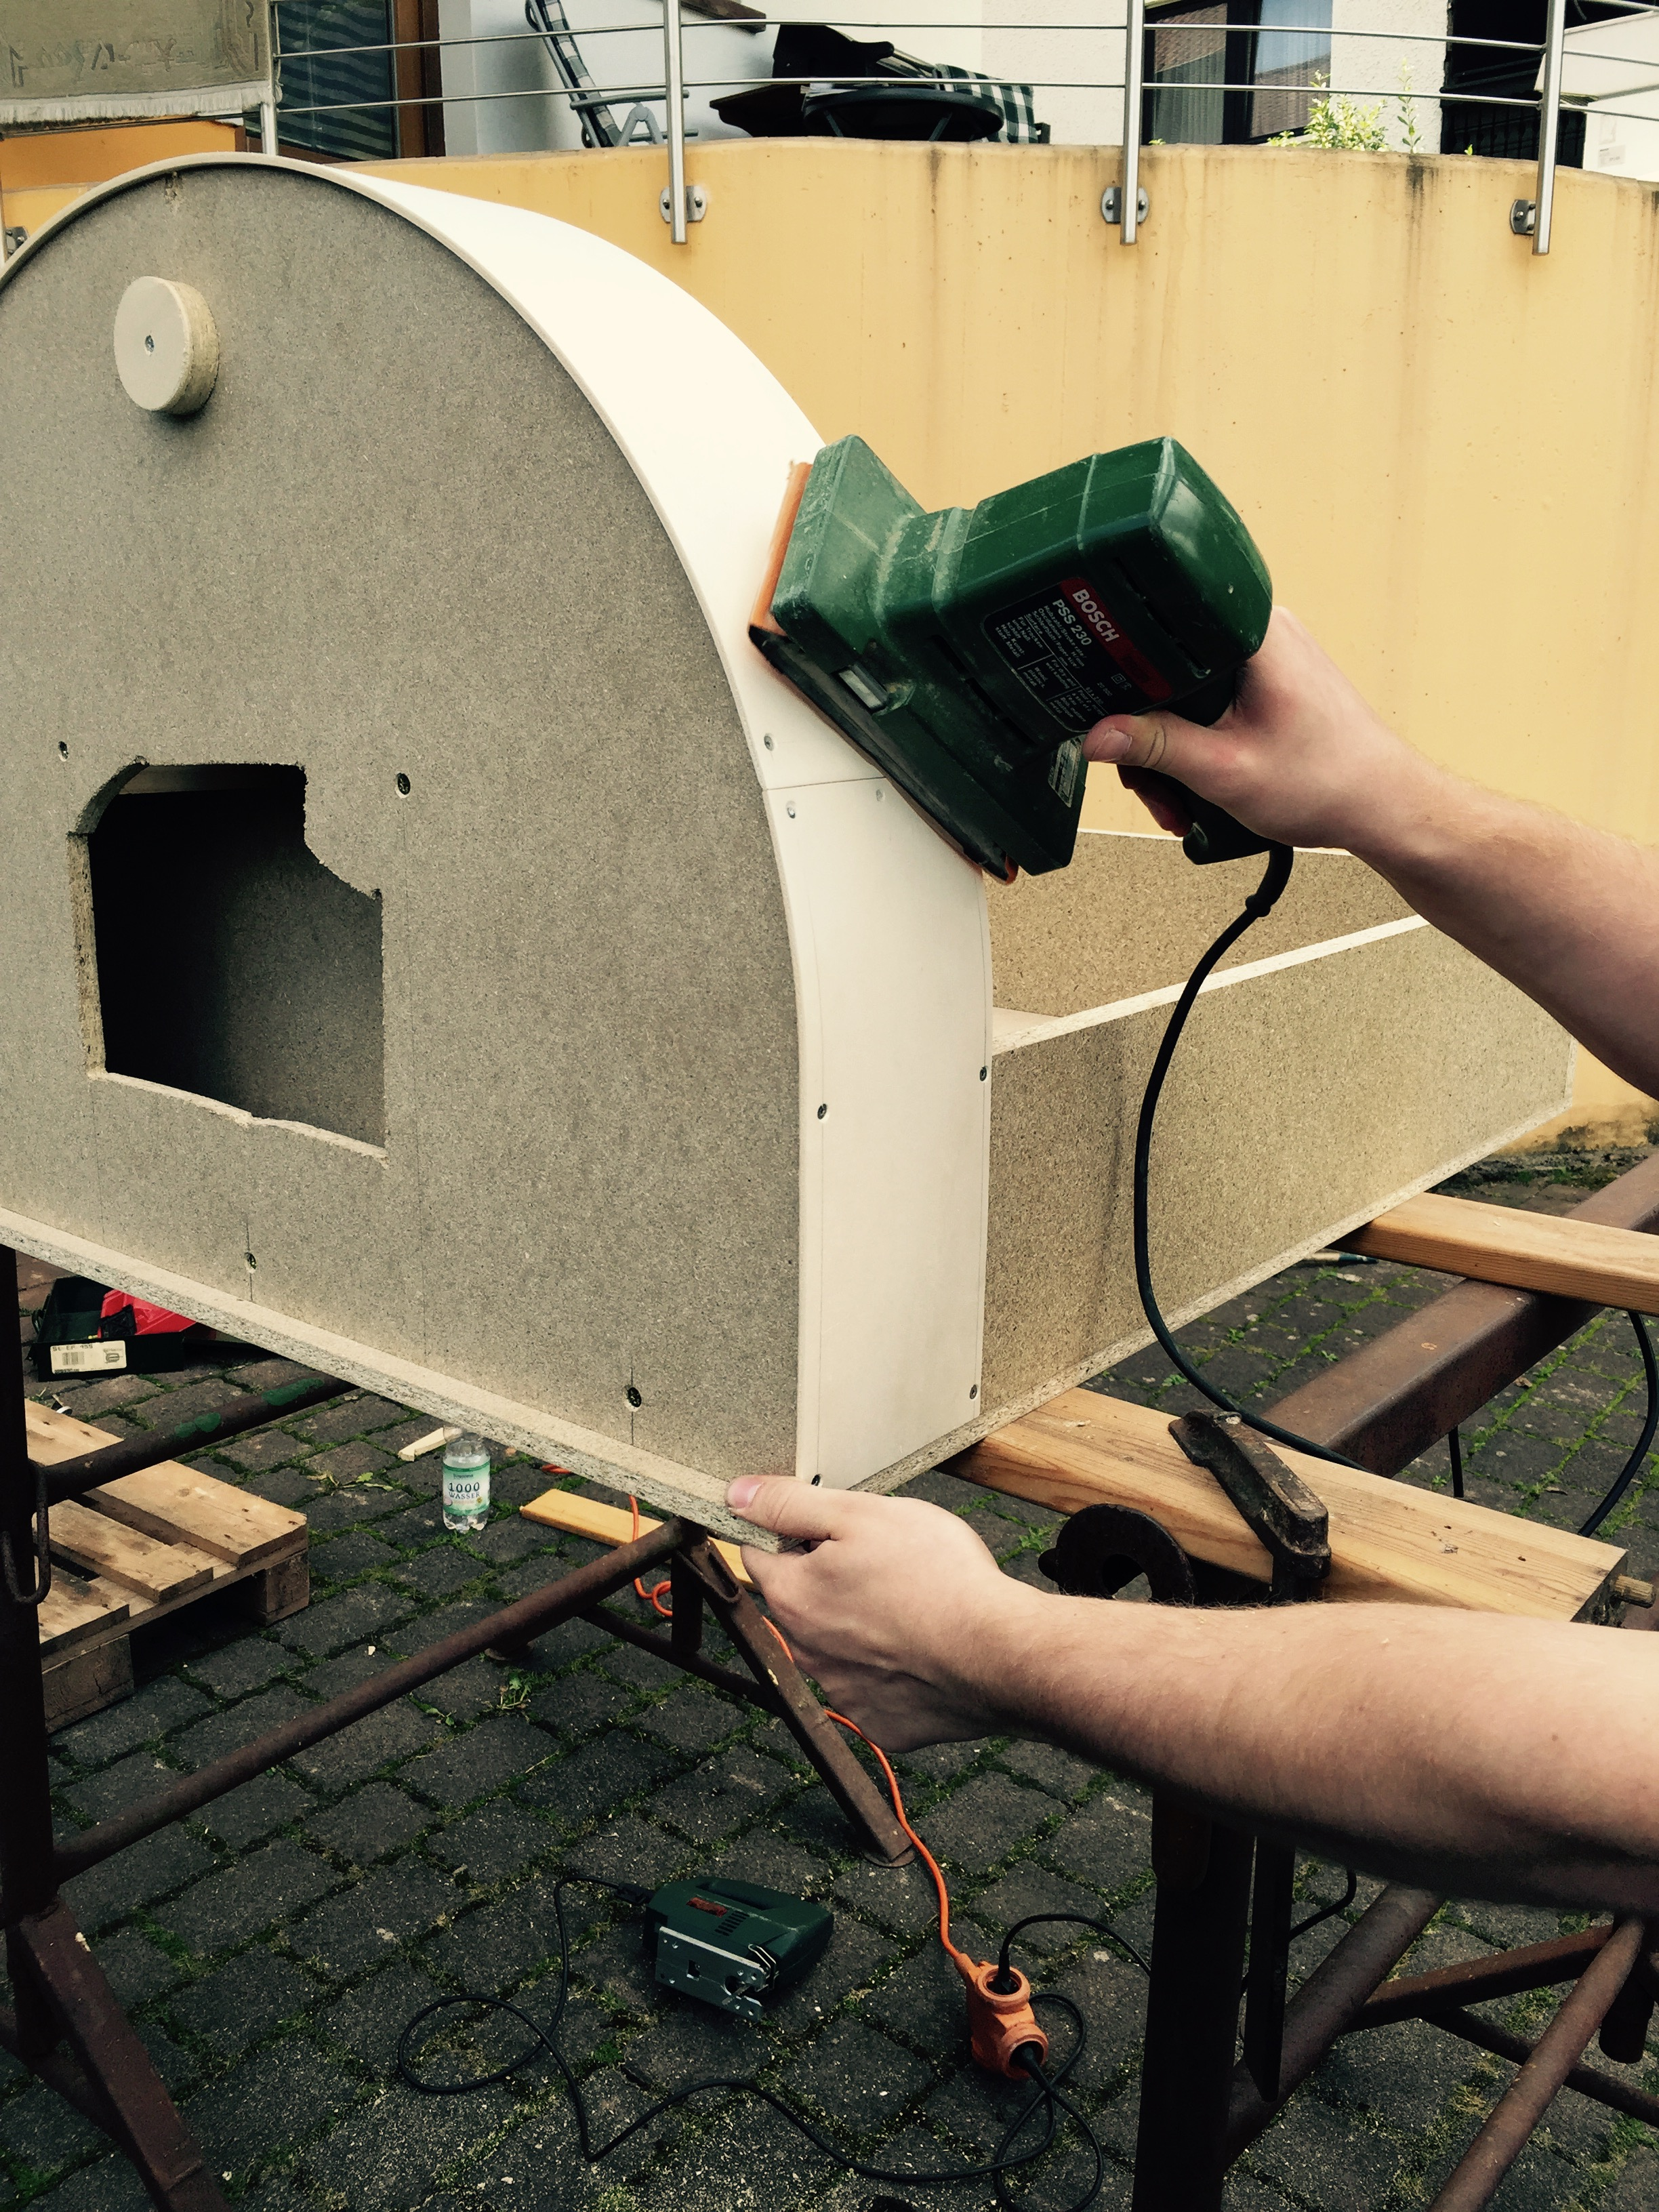
\includegraphics[width=0.5\linewidth]{pictures/polishing.jpg}
  \caption{Polishing the rack}
  \label{fig:polishing}
\end{figure}

After polishing and cleaning the rack with compressed air, we were able to prime the rack. This is important since primer creates a smooth and consistent layer for the paint.

\begin{figure}[htbp] 
  \centering
     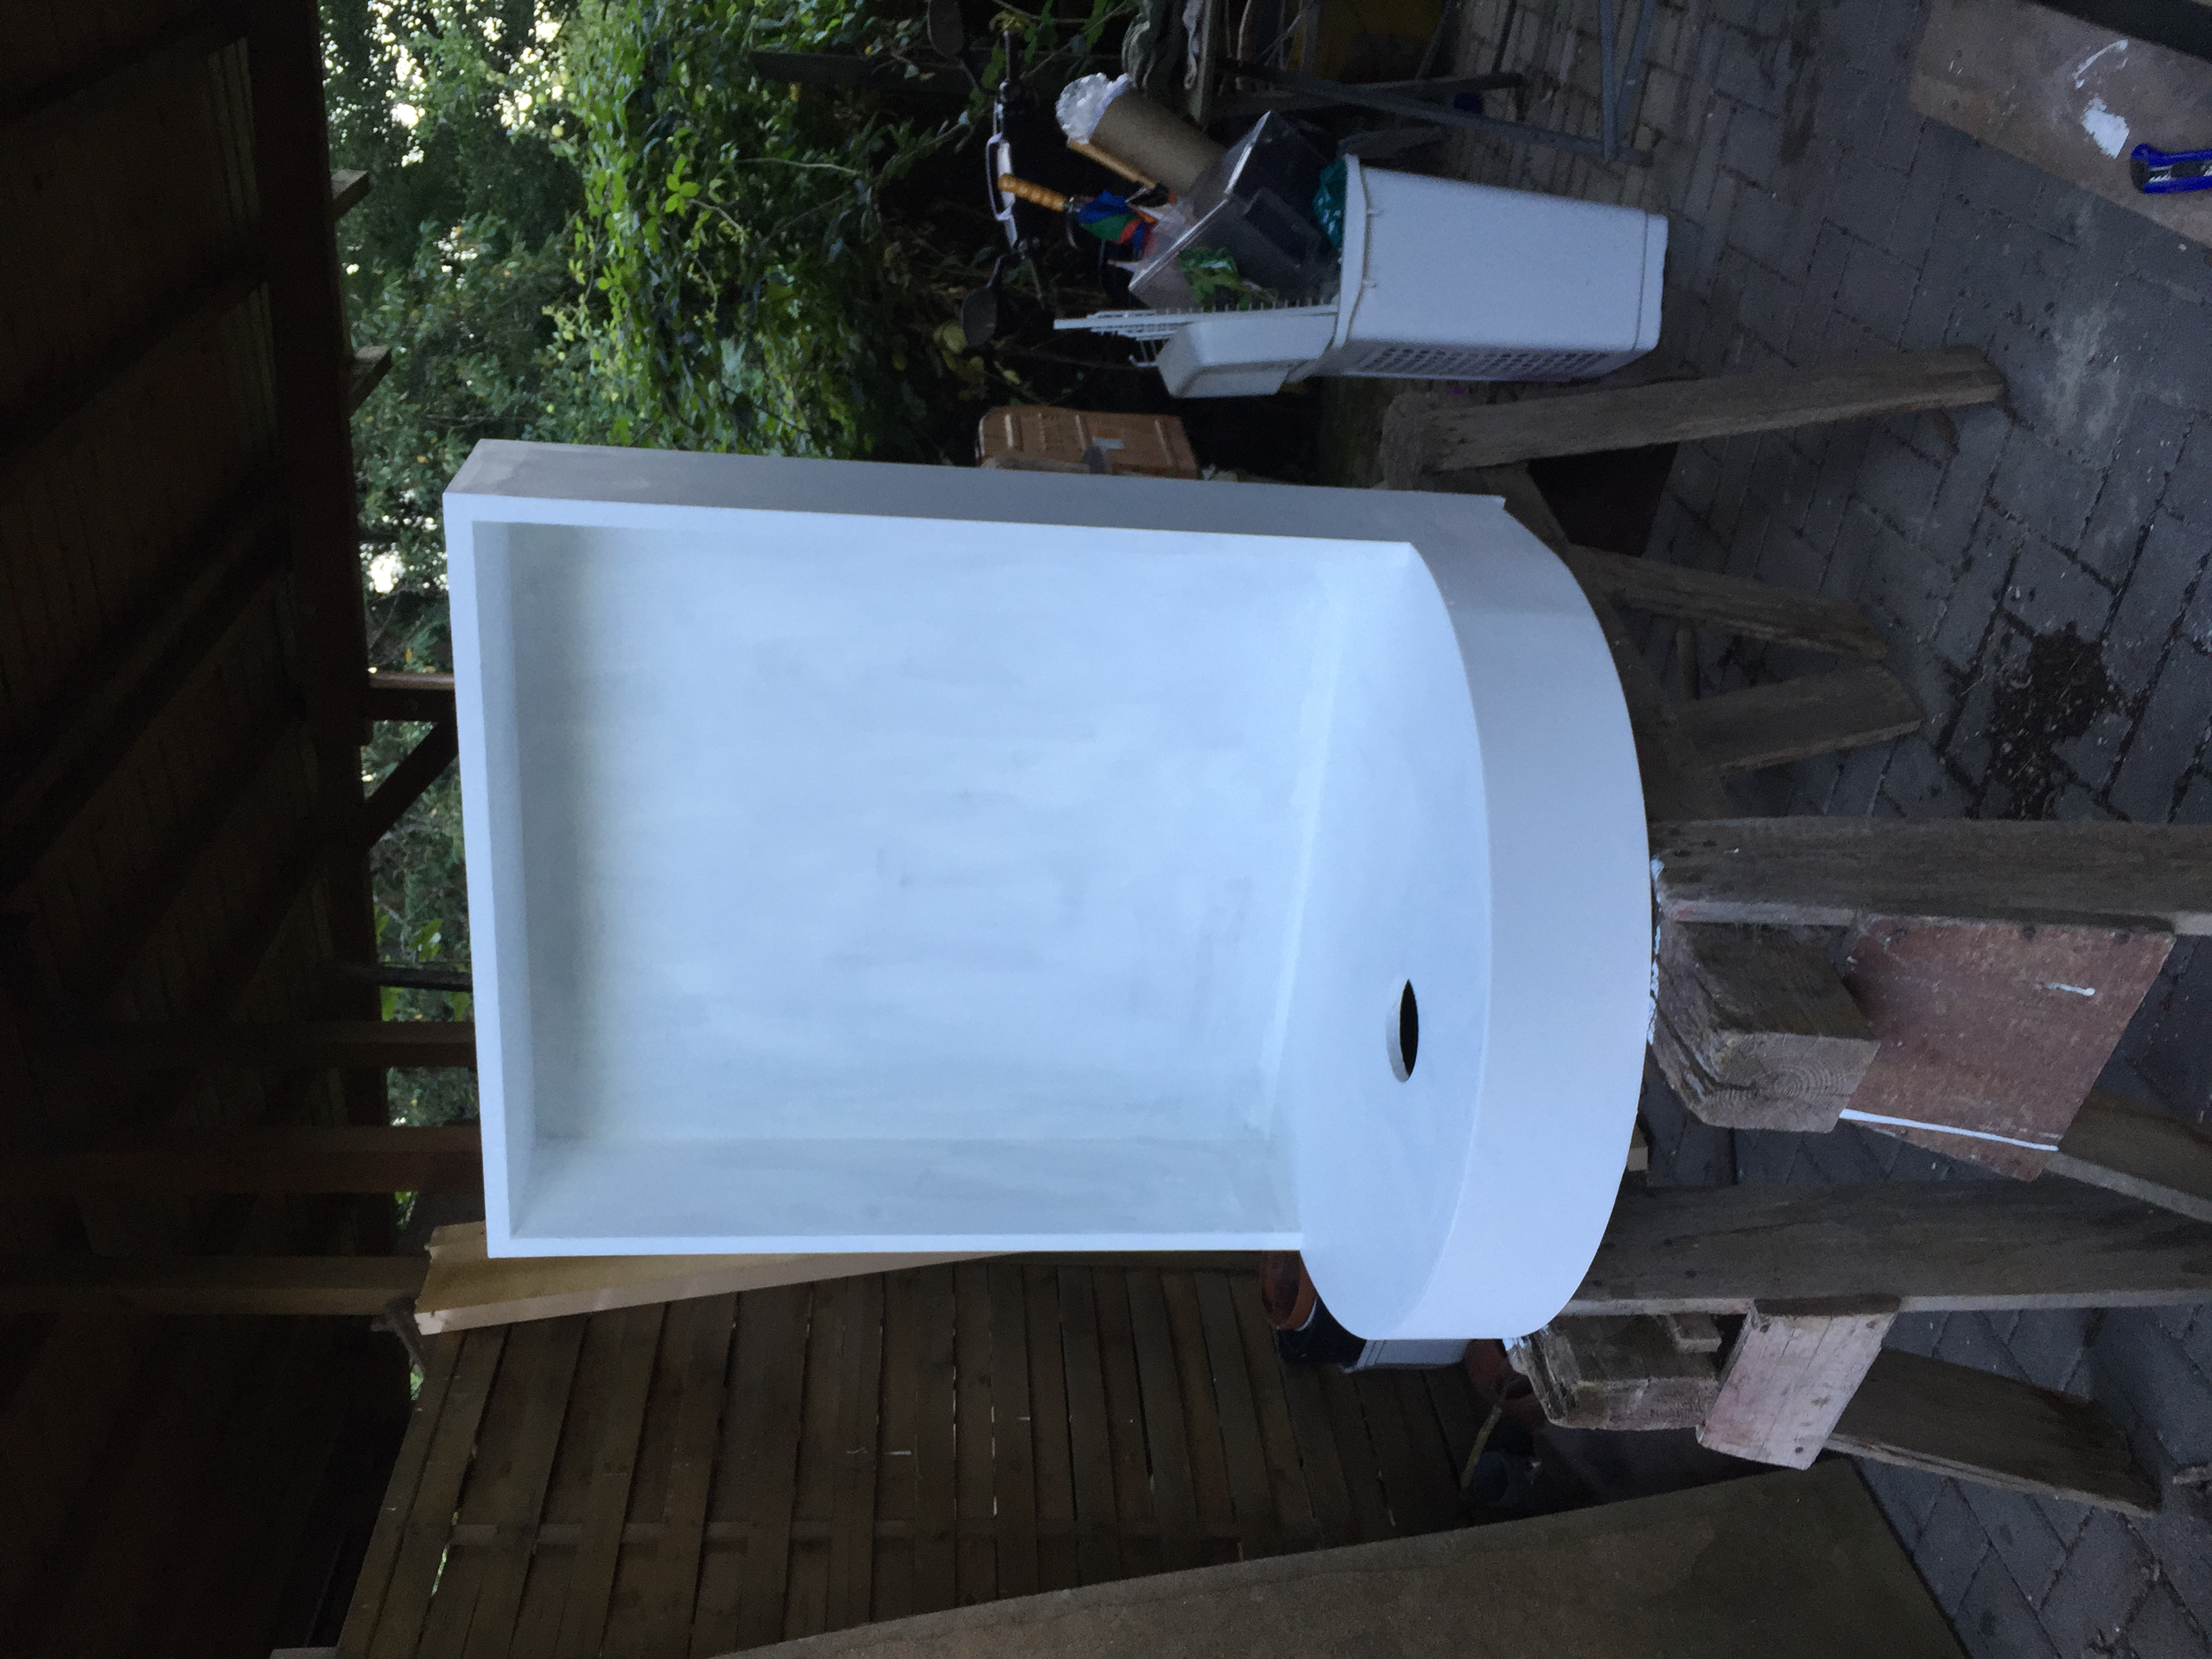
\includegraphics[width=0.6\linewidth, angle =270]{pictures/rack3.jpg}
  \caption{The primed rack}
  \label{fig:priming}
\end{figure}



\subsection{Acrylic Glass}

\begin{figure}[htbp] 
  \centering
     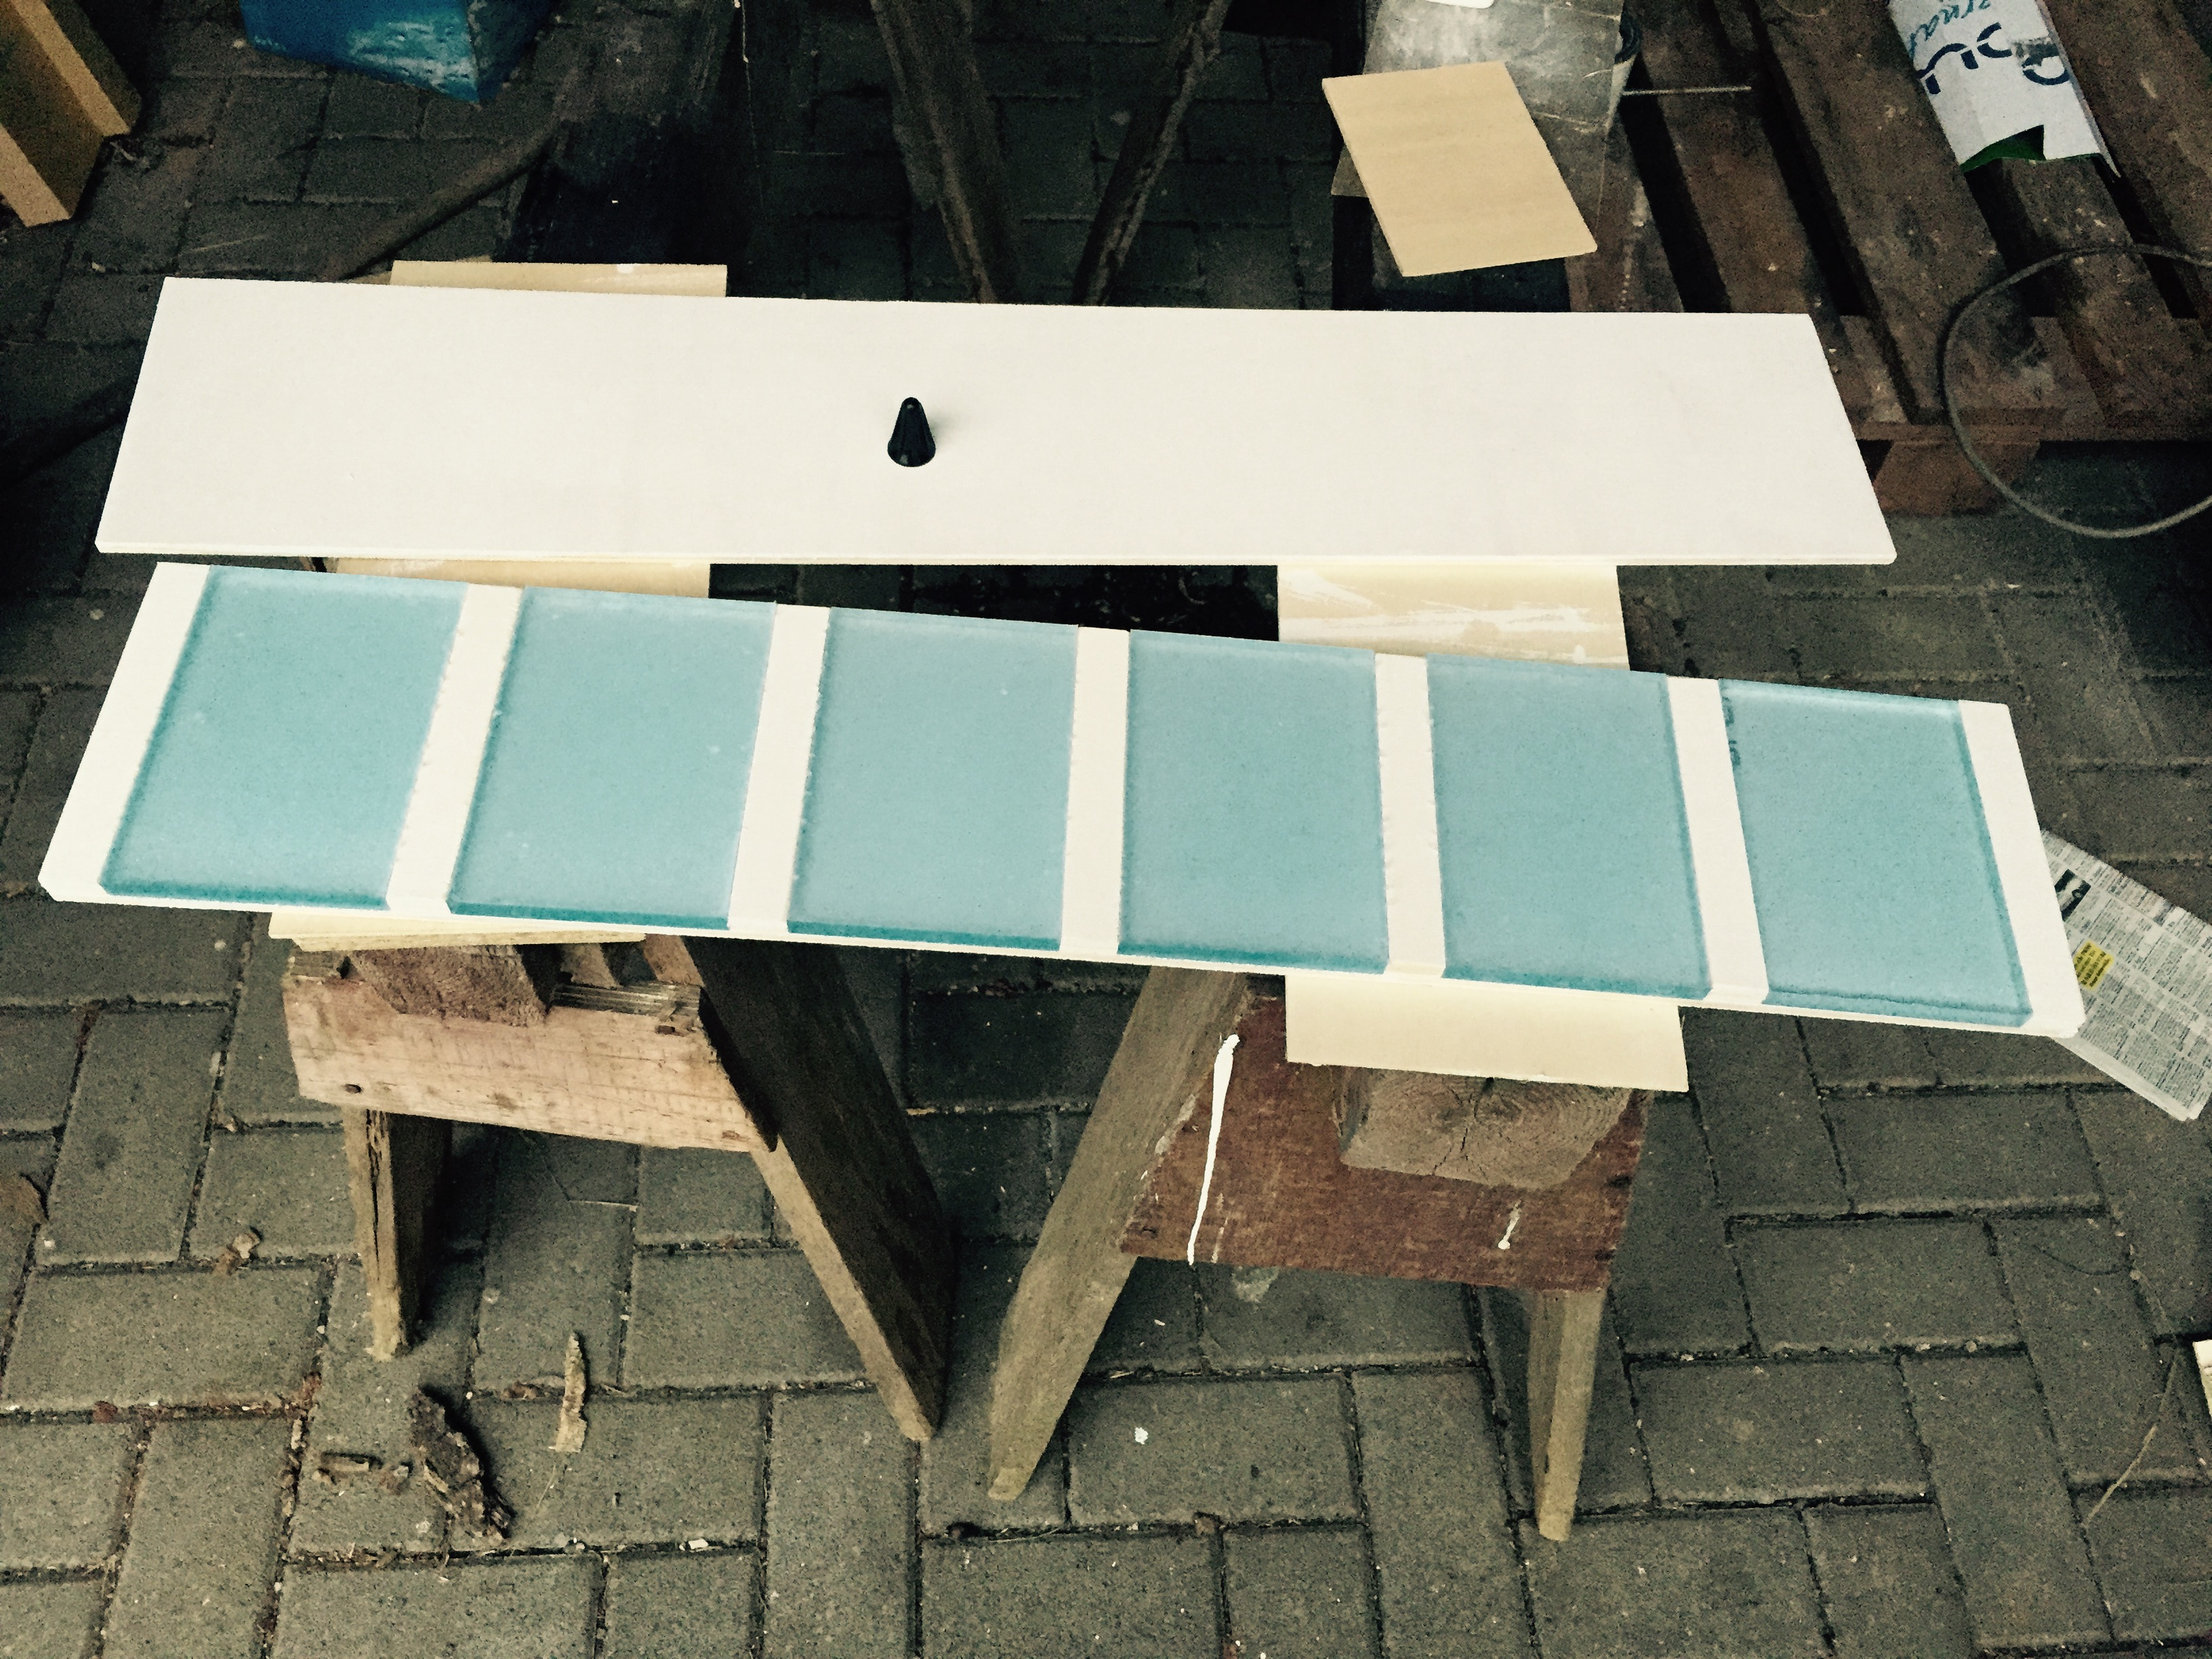
\includegraphics[width=0.5\linewidth]{pictures/plexiglass.jpg}
  \caption{Building the shelves}
  \label{fig:building_shelves}
\end{figure}

\begin{figure}[htbp] 
  \centering
     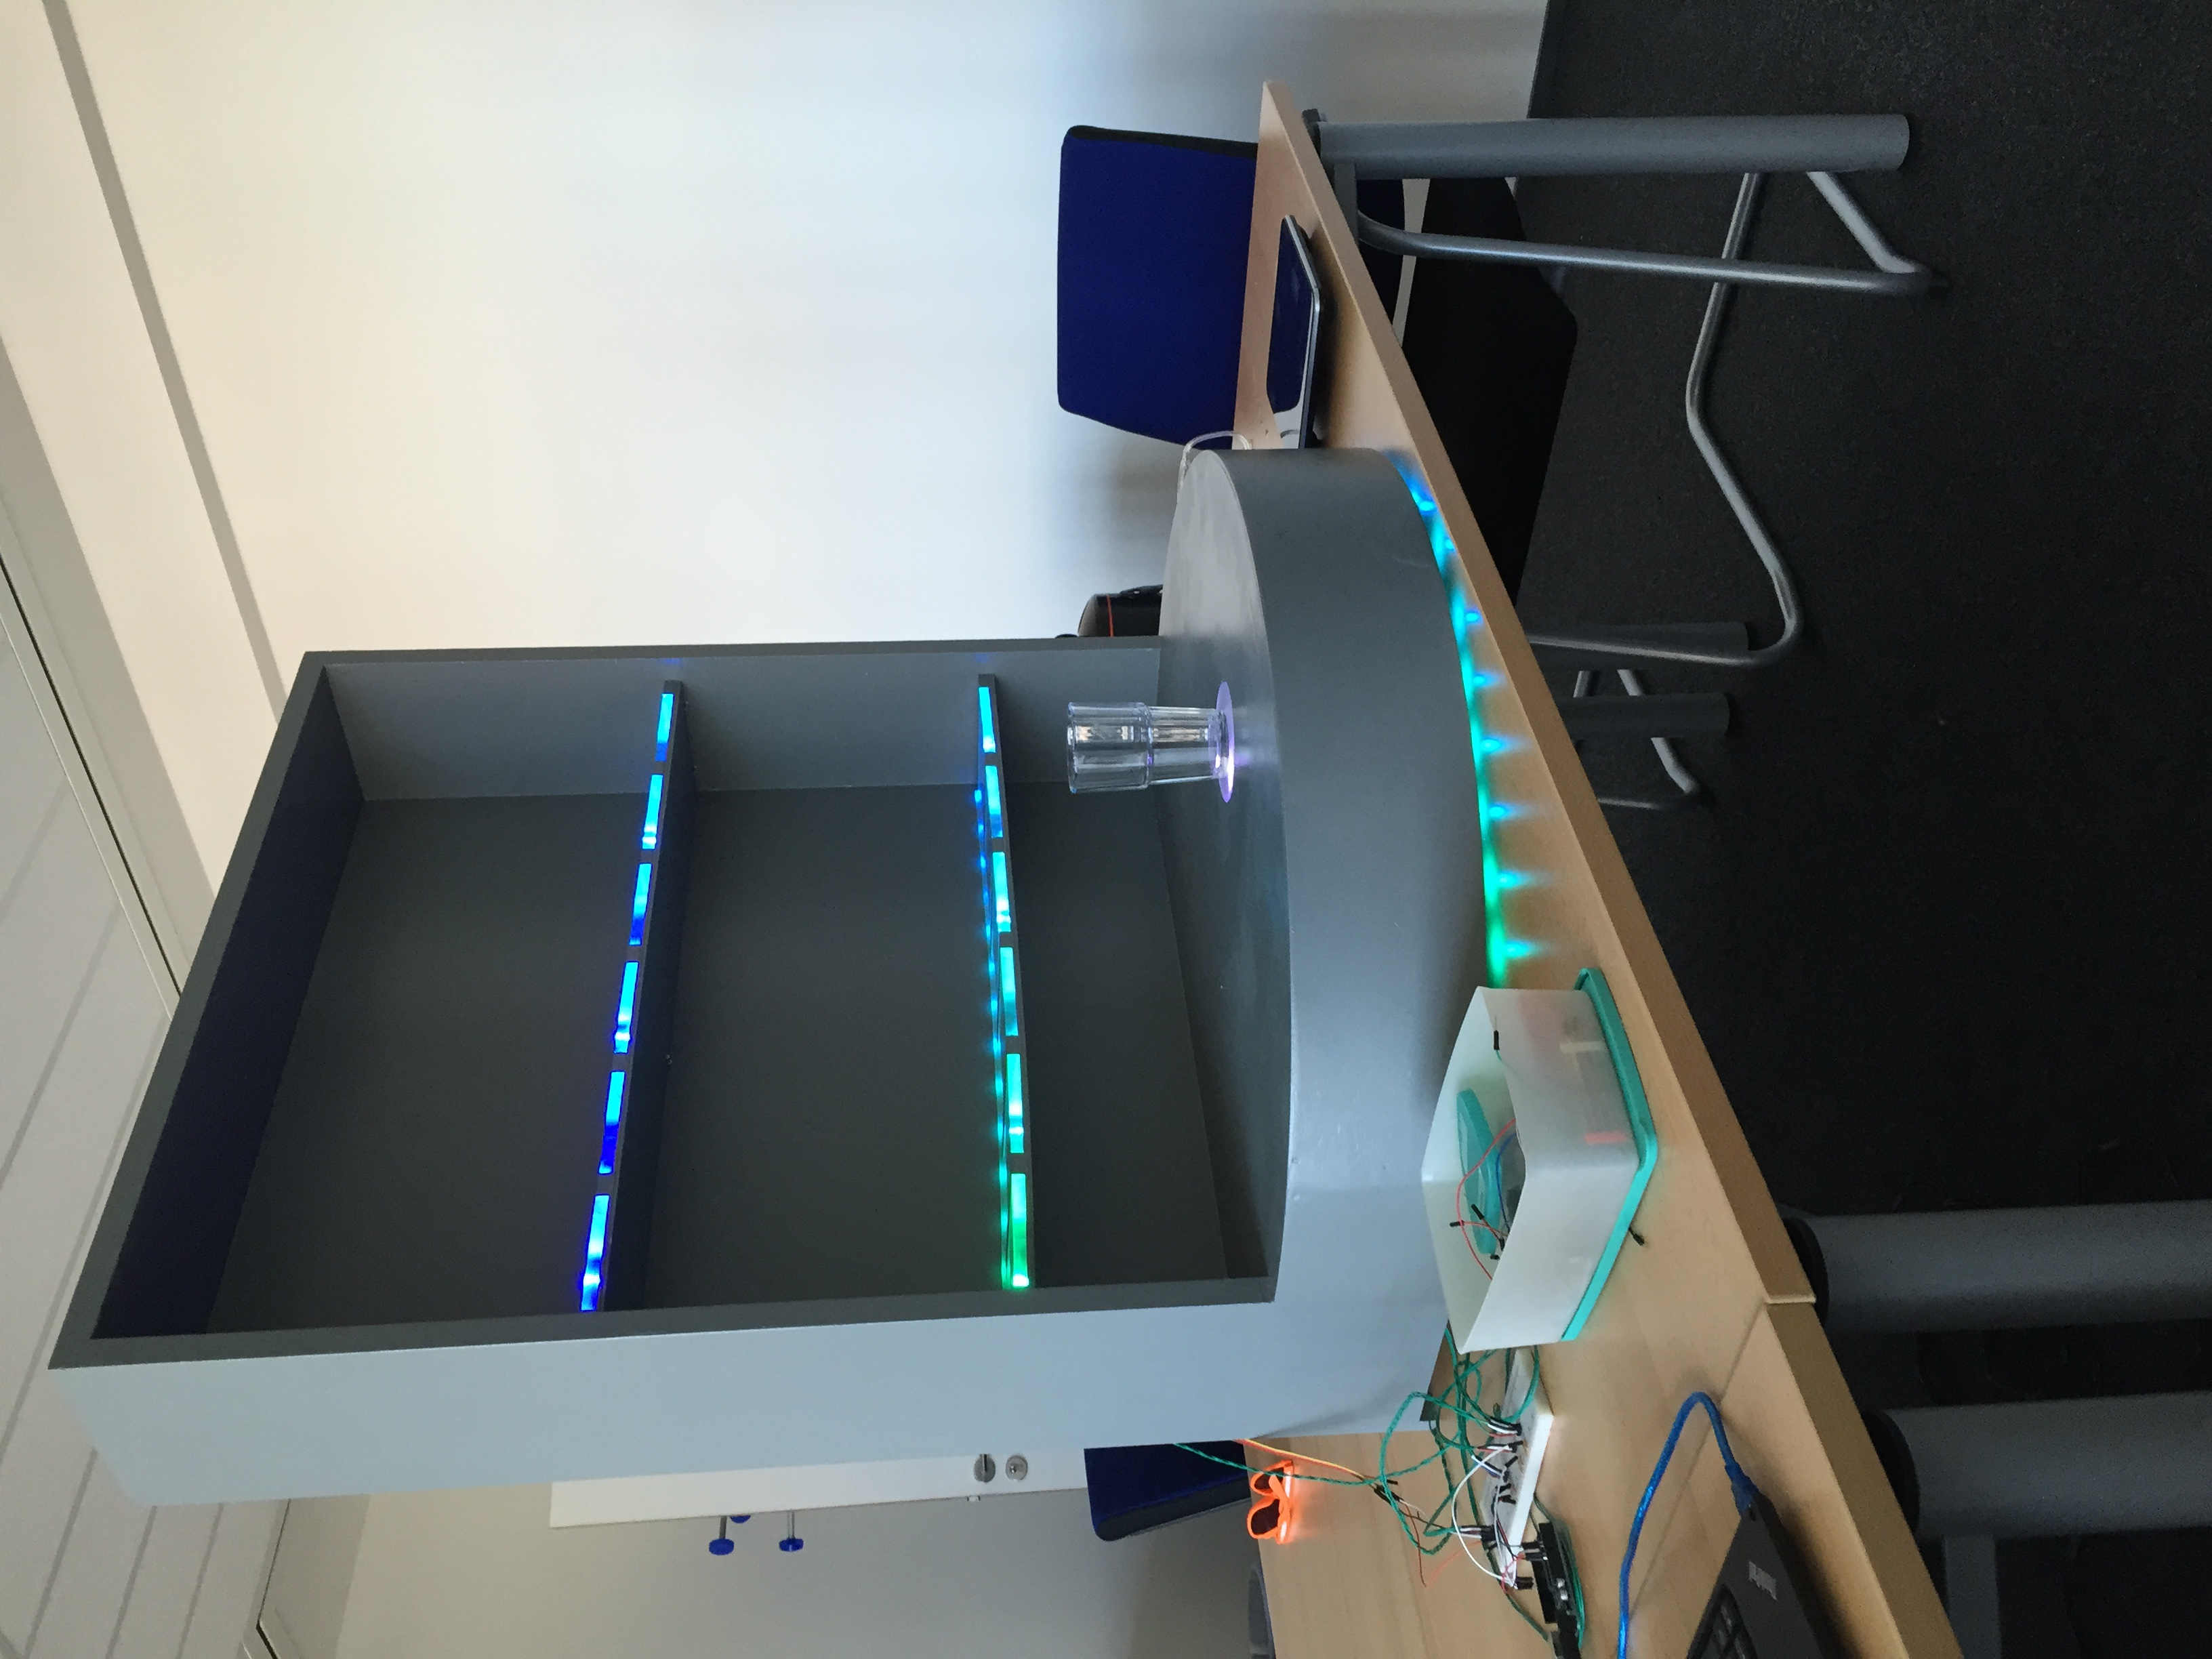
\includegraphics[width=0.5\linewidth]{pictures/iluminated_shelves.jpg}
  \caption{Building the shelves}
  \label{fig:iluminated_shelves}
\end{figure}


\subsection{Soldering and Wiring}
Finally we needed to connect all electronic parts together. The Raspberry Pi and the Arduino Uno are connected via an standard USB cable. Both have an individual 5 Volt power adapter with 1.2 Ampere for the Arduino and ? Ampere for the Raspberry Pi. We have 5 LED stripes: One for both shelves, one for the glasses, one for the shaker and the ice, one for the glass panel above the scale and one for floor illumination. Each stripe needs three connections, one to ground, one to 5 Volt and one data connection to a digital pin the Arduino board. The scale is connected to a weighting module which is also connected to ground and 5 Volt and additional to 2 analog inputs on the Arduino board.

All cables are equipped with plugs for easier assembling. For the LED stripes they were neccesary as the stripes doesn't fit through the drill holes. The cables from the stripes and the weighting module are all plugged into a circuit board, which itself connects to the Arduino with only 3 plugs. 

\section{Software Construction}
\subsection{Raspberry Pi and Arduino}
\subsection{Webserver}
\label{sec:webserver}
\subsection{Database}
\subsection{Communication}
\section{User Guide}
\subsection{Start the System}
To start the system you just need to connect the bar to the power supply system. After that the Raspberry Pi boots and when the 'Bar Dude' website is displayed, you can start ordering your cocktails.
\subsection{Select a Cocktail}
You have to connect to the Access Point 'CocktailPi' and log in with the password 'CocktailPi'. Then go to '192.168.0.1' in your browser. Now you can see the interface where you can choose your cocktail. For more information about the website read section \ref{sec:webserver}. You choose your cocktail by clicking on the corresponding 'Do it dude!' button. You get a number to know which cocktail is your's.
\subsection{Mix the Cocktail}
When your number is displayed on the display of the Raspberry Pi, you have 30 seconds to touch the weight measuring module. It also displays the countdown. If the time runs out, the order is deleted and the next cocktail number is displayed. \\
Now you can follow the instructions of the display. First you have to take a glass or a shaker depending on which is illuminated and put it on the weight measuring module. Then you add the illuminated ingredients. The weight measuring module shows you which amount if the ingredient is needed. It changes the color from red to green and the speed of the illumination slows down until you fill in enough. If you use a shaker you have to shake it when the bar goes wild. Then you have to take a glass and fill the content of the shaker into the glass. If you take a glass at first, you normally, not always, have to mix your cocktail. In this case the weight measuring module displays a circle. Take a spoon and mix until the next step is displayed. When your cocktail is finished, a party mode is displayed. 

\section{Conclusions}


%\section{Acknowledgments}
%This section is optional; it is a location for you
%to acknowledge grants, funding, editing assistance and
%what have you.  In the present case, for example, the
%authors would like to thank Gerald Murray of ACM for
%his help in codifying this \textit{Author's Guide}
%and the \textbf{.cls} and \textbf{.tex} files that it describes.

\end{document}
